When messing with malware on your machine I figured I would either want
to run it in a VM or make sure none of the prerequisites are enabled on
the machine itself. This is where malware written in C or C++ thrive as
languages like Python and Java need the runtime and interpreter already
installed to meet that prerequisite. For this assignment I decided to
take a look at the Zeus trojan malware pkg that initially gaining
traction in the late 2000s when used to streal info from the US DoT.
Trojans are known to be malware that behaves as legitimate programs. The
bot would go on to infecting millions of computers and spawning any
variants. The bot is aimed to target windows machines to extract banking
informations using keystroke logging. This form of attack is a common
example of a man-in-the-middle attack. The malware pkg performs
infection via phishing schemes or drive-by downloads and infected some
of the largest companies such as Bank of America, Oracle, Cisco, Amazon,
etc. The trojan violates just about every principle in the CIA triad.
Since confidential banking information was taken as well as money,
confidentially and integrity are both violated while availability
remains in questions. Patches to the malware offered from cybersecurity
consultants is known to eradicate it from the infected machine, however
strains of the virus were spawned remaining a constant battle.

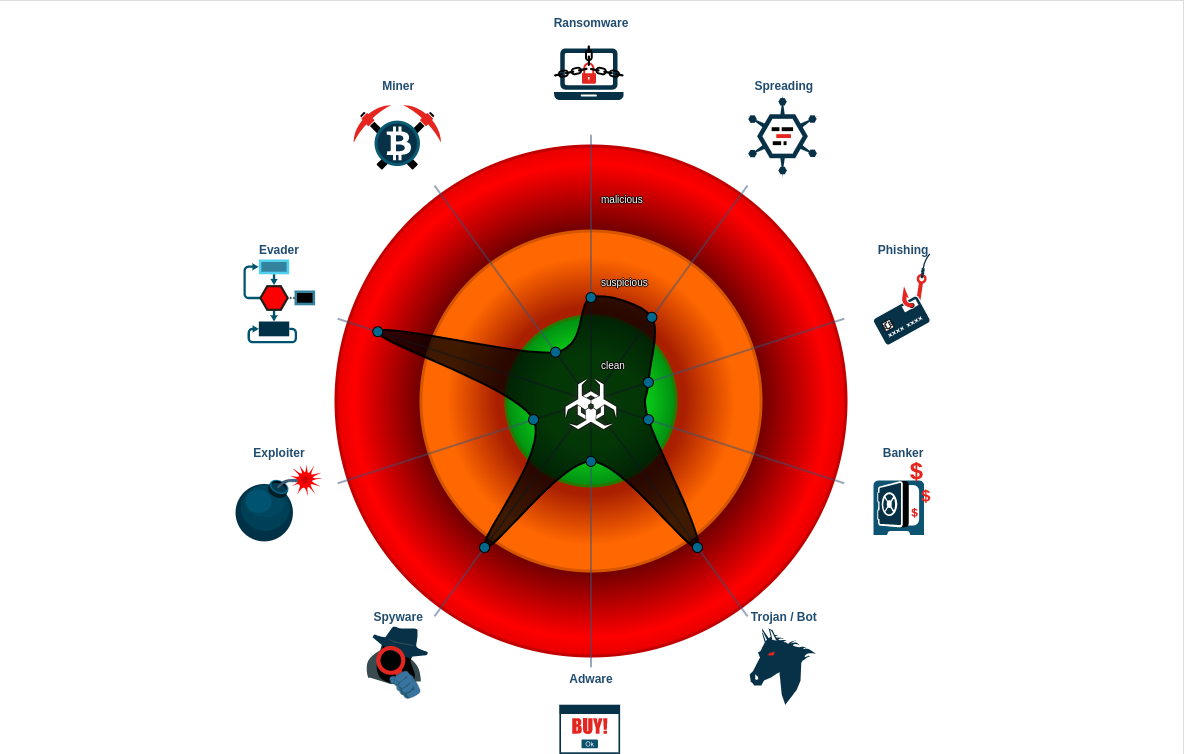
\includegraphics{https://github.com/akielaries/CYB410-secure-software/blob/main/imgs/ZEUS_CLASSIFICATION.png}

I was able to find several versions of the "leaked" banking trojan but
check out the version I had found from here!

\href{https://github.com/touyachrist/evo-zeus}{https://github.com/touyachrist/evo-zeus}

Although not the most dentrimental part of the source code, in a repo
containing the Zeus source code this block minimally shows the entry
point to the windows core API was created and giving root permission

\begin{Shaded}
\begin{Highlighting}[]
\DataTypeTok{void}\NormalTok{ WINAPI entryPoint(}\DataTypeTok{void}\NormalTok{) \{}
\NormalTok{  Mem::init();}
\NormalTok{  Console::init();  }
\NormalTok{  Crypt::init();}
\NormalTok{  Core::init();}
  
\NormalTok{  CUI\_DEFAULT\_COMMANDLINE\_HELPER;}

\NormalTok{  Core::uninit();}
\NormalTok{  Crypt::uninit();}
\NormalTok{  Console::uninit();}
\NormalTok{  Mem::uninit();}
  
\NormalTok{  CWA(kernel32, ExitProcess)(coreData.exitCode);}
\NormalTok{\}}
\end{Highlighting}
\end{Shaded}

A similar version of this code I ran on my machine running kali linux,
was able to give me root permissions as a regular user. See here (maybe
it works for you):

\begin{Shaded}
\begin{Highlighting}[]
\DataTypeTok{int}\NormalTok{ getuid()\{}
    \ControlFlowTok{return} \DecValTok{0}\NormalTok{;}
\NormalTok{\}}
\DataTypeTok{int}\NormalTok{ geteuid()\{}
    \ControlFlowTok{return} \DecValTok{0}\NormalTok{;}
\NormalTok{\}}
\DataTypeTok{int}\NormalTok{ getgid()\{}
    \ControlFlowTok{return} \DecValTok{0}\NormalTok{;}
\NormalTok{\}}
\DataTypeTok{int}\NormalTok{ getegid()\{}
    \ControlFlowTok{return} \DecValTok{0}\NormalTok{;}
\NormalTok{\}}

\end{Highlighting}
\end{Shaded}

The bot has went thru many stages and versions with earlier versions of
the bug had executable files hardcoded to one of these files

\begin{verbatim}
ntos.exe
oembios.exe
twext.exe
\end{verbatim}

date being stored in the folowing dirs

\begin{verbatim}
System>\wsnpoem 
System>\sysproc64
System>\twain_32
\end{verbatim}

the next iteration and stored files in a single directory later found by
security researchers, with another version storing executables in
randomly named folders in app data.

The bot executes in the following stages

\begin{itemize}
\item
  Builder This malware comes in a kit usable by regular users with no
  technical knowledge, meaning the "owner" must deploy their own
  executables to who they wish to infect. This is done easily by using
  the builder in the tool kit. Each build will be unique to the
  infectee, due to some cryptographic implementations, there are uniquie
  keys generated for the configuration file embedded into the built
  .exe.
\item
  Configuration Seperate from the build stage, contains the address to
  where the sniffed data is sent to in a series of blocks enables
  customization and hardcoding settings into the final binary. The
  config includes these sections:
\end{itemize}

\begin{verbatim}
StaticConfig 
DynamicConfig
KeyLogger
WebFilters
WebDataFilters
WebFakes
\end{verbatim}

Static and Dynamic Config both are dealing with the hardcoding of
settings that eventually get executed at runtime. Here the questions of
what is the target and destination get answered. In addition to the
hardcoding of generic settings, dynamic features that imply additional
comlexity such as redirection URLs of targets and destination addresses,
URL masks, log disabling, sets of URLs performing Transaction
Authenticaion Number (TAN) harvesting, as well as URL maks that contain
corresponding HTML blocks injecting into webpages who match the
Webinjects requests. The bot is responsible for running queries

Example of the config.txt file used to initate seen here:
\href{https://github.com/touyachrist/evo-zeus/blob/master/output/builder/config.txt}{https://github.com/touyachrist/evo-zeus/blob/master/output/builder/config.txt}

Example of webinjects.txt file used to targeting:
\href{https://github.com/touyachrist/evo-zeus/blob/master/source/other/webinjects.txt}{https://github.com/touyachrist/evo-zeus/blob/master/source/other/webinjects.txt}

\begin{itemize}
\item
  Execution The final executable file produced from build and configure
  (sounds like installing a C application) is finally deployed by the
  "owner" of the bug. If the .exe is produced with the same cofiguration
  and build settings the end results will usually vary in where the
  config file is stored.
\item
  Server Finally the bot is deployed on a php-based server utilized by
  an abundance of php scripts that allows the deployer to monitor their
  results! This also serves as a sort of remote access type application
  where CMDs can be issued using this stage.
\item
  Why wasn't it detected? From its initial release, the bot itself was
  made more complex and harder to detect for a number a reasons. What
  made things tricky was random naming of files to specific directories
  and in small sizes. Using checksums is monitoring bits transmitted at
  a higher rate than normal, letting professionals know of some
  potential issues. In earlier stages the bug transmitted files
  carelessly and copied them into the system dir. Later versions made
  use of ensuring dropped files were not to have the same checksum as
  the orignal.
\end{itemize}

The general function of the bug is to continuously spawn threads based
on previous ones that go around crawling the infected devices hard
drive. Doing so by embedding itself into system directories.

Here we can see in assembly code how finding new executables to download
content. The config file is written into our registers and that same
thread it is executed in will attempt to scrape for new .exe files for
config to point to.

Here is an example of how the keylogging and screens scraping takes
place by importing a hook to the API

\begin{verbatim}
user32!TranslateMessage
\end{verbatim}

If the a left click is detected, a global flag is set within another PAI
hook and another check is conducted to check if the user is visiting a
location specified in the config file. Screen captures are then only
taken when visiting what is specified by the creator. This uses win32
functions that can also be seen here:
\href{https://github.com/touyachrist/evo-zeus/blob/master/source/client/screenshot.cpp}{https://github.com/touyachrist/evo-zeus/blob/master/source/client/screenshot.cpp}

\begin{Shaded}
\begin{Highlighting}[]
\NormalTok{HDC hDC = CreateCompatibleDC(}\DecValTok{0}\NormalTok{);}
\NormalTok{HBITMAP hBmp = CreateCompatibleBitmap(GetDC(}\DecValTok{0}\NormalTok{), screen\_width,}
\NormalTok{screen\_height);}
\NormalTok{SelectObject(hDC, hBmp);}
\NormalTok{BitBlt(hDC, }\DecValTok{0}\NormalTok{, }\DecValTok{0}\NormalTok{, screen\_width, screen\_height, x\_coordinate,}
\NormalTok{y\_coordinate, SRCCOPY); }
\end{Highlighting}
\end{Shaded}

Lets also take a look at the differences in a small implementation of
the RC4 stream cipher in a early and more recent version

The difference being the second implementation is encrypting the config
file a 0x100 byte key at build time. An extra layer scen in v2 adds more
complexity by implementing a XOR decryption (last code block)

\begin{Shaded}
\begin{Highlighting}[]
\CommentTok{/*}
\CommentTok{ * Example of config file encryption seen in v1}
\CommentTok{ */}

\NormalTok{dataSize = size of data}
\NormalTok{dataIn = encrypted data}
\DataTypeTok{char}\NormalTok{ b;}
    \ControlFlowTok{for}\NormalTok{ (i = }\DecValTok{0}\NormalTok{; i \textless{} dataSize; i++) \{}
\NormalTok{        dataOut[i] = }\DecValTok{0}\NormalTok{;}
\NormalTok{    \}}
    \ControlFlowTok{for}\NormalTok{ (i = }\DecValTok{0}\NormalTok{; i \textless{} dataSize; i++) \{}
\NormalTok{        b = dataIn[i];}
        \ControlFlowTok{if}\NormalTok{ ((i \% }\DecValTok{2}\NormalTok{) == }\DecValTok{0}\NormalTok{) \{}
\NormalTok{            b += }\DecValTok{2}\NormalTok{ * i + }\DecValTok{10}\NormalTok{;}
\NormalTok{        \}}
        \ControlFlowTok{else}\NormalTok{ \{}
\NormalTok{            b += }\BaseNTok{0xF9}\NormalTok{ {-} }\DecValTok{2}\NormalTok{ * i;}
\NormalTok{        \}}
\NormalTok{        dataOut[i] += b;}
\NormalTok{    \}}

\end{Highlighting}
\end{Shaded}

\begin{Shaded}
\begin{Highlighting}[]
\CommentTok{/*}
\CommentTok{ * A look at v1.x encryption on config files}
\CommentTok{ */}

\DataTypeTok{int}\NormalTok{ rc4\_decrypt(}\DataTypeTok{unsigned} \DataTypeTok{char}\NormalTok{ *in, }\DataTypeTok{unsigned} \DataTypeTok{long}\NormalTok{ size, }
    \DataTypeTok{unsigned} \DataTypeTok{char}\NormalTok{ *S, }\DataTypeTok{unsigned} \DataTypeTok{char}\NormalTok{ *out) \{}
    \DataTypeTok{int}\NormalTok{ i, j, dataCount;}
\NormalTok{    i = j = dataCount = }\DecValTok{0}\NormalTok{;}
    \DataTypeTok{unsigned} \DataTypeTok{char}\NormalTok{ temp, rc4\_byte;}
    \ControlFlowTok{for}\NormalTok{ (dataCount = }\DecValTok{0}\NormalTok{; dataCount \textless{} size; dataCount++) \{}
\NormalTok{        i = (i + }\DecValTok{1}\NormalTok{) \& }\DecValTok{255}\NormalTok{;}
\NormalTok{        j = (j + S[i]) \& }\DecValTok{255}\NormalTok{;}
\NormalTok{        temp = S[j];}
\NormalTok{        S[j] = S[i];}
\NormalTok{        S[i] = temp;}
\NormalTok{        rc4\_byte = S[(temp + S[j]) \& }\DecValTok{255}\NormalTok{];}
\NormalTok{        out[dataCount] = in[dataCount] \^{} rc4\_byte;}
\NormalTok{    \}   }
    \ControlFlowTok{return}\NormalTok{ dataCount;}
\NormalTok{\} }

\end{Highlighting}
\end{Shaded}

\begin{Shaded}
\begin{Highlighting}[]
\ControlFlowTok{for}\NormalTok{ (m = (decSize{-}}\DecValTok{1}\NormalTok{); m \textgreater{}}\DecValTok{0}\NormalTok{; m{-}{-}) \{}
\NormalTok{    decData[m] = decData[m]\^{} decData[m{-}}\DecValTok{1}\NormalTok{];}
\NormalTok{    \}}
\end{Highlighting}
\end{Shaded}

\hypertarget{further-look-at-rc4-encryption--static-analysis-w-clang}{%
\section{Further Look at RC4 Encryption + Static Analysis w/
CLang}\label{further-look-at-rc4-encryption--static-analysis-w-clang}}

The RC4 Stream Cipher was an encryption algorithm used in many Windows
systems for a variety of applications. The Zeus bot exploited this
algorithm and went under a series of patches (for example using logical
operator XOR to swap instead of int/ char method)

We will take a look at how the cipher is implemented for small scale use
(passing in a key, string, expecting a returned hash). The analysis on
this isn't very exciting and was not implemented by the attackers but
exploited by them. The errors in the RC4 algorithms are beyond what I
beleive will be caught by a static analysis tool like CLang. Running the
windows-based bug on my linux machine was troublesome with CLange so I
had decided to look at a more broad issues that contributed to the bug.

So we will be looking at a minimal reproducable problem for catching
bank statements from the system.

\hypertarget{rc4-v0c}{%
\paragraph{rc4-v0.c}\label{rc4-v0c}}

ITER 1 :

\begin{verbatim}
$ ./rc4-v0 1 hello
087FAE01F8

KEY = 1
STRING = hello
HASH = 087FAE01F8
\end{verbatim}

ITER 2 :

\begin{verbatim}
$ ./rc4-v0 1 HELLO
285F8E21D8

KEY = 1
STRING = HELLO
HASH = 285F8E21D8
\end{verbatim}

ITER 3 :

\begin{verbatim}
$ ./rc4-v0 224 secure_software
F96FCDD6802CC1F80298D5C5439B26

KEY = 224
STRING = secure_software
HASH = F96FCDD6802CC1F80298D5C5439B26
\end{verbatim}

ITER 4 :

\begin{verbatim}
$ ./rc4-v0 int too
28BEF0

KEY = int
STRING = too
HASH = 28BEF0
\end{verbatim}

Produces different hash based on case-type

\textbf{Static Analysis}

\begin{Shaded}
\begin{Highlighting}[]
\NormalTok{clang {-}{-}analyze rc4{-}v0.c}
\NormalTok{rc4{-}v0.c:}\DecValTok{72}\NormalTok{:}\DecValTok{33}\NormalTok{: warning: Result of \textquotesingle{}malloc\textquotesingle{} is converted to a pointer}
\NormalTok{of type \textquotesingle{}}\DataTypeTok{unsigned} \DataTypeTok{char}\NormalTok{\textquotesingle{}, which is incompatible with }\KeywordTok{sizeof}\NormalTok{ operand type}
\DataTypeTok{int}\NormalTok{\textquotesingle{} [unix.MallocSizeof]}
    \DataTypeTok{unsigned} \DataTypeTok{char}\NormalTok{ *ciphertext = malloc(}\KeywordTok{sizeof}\NormalTok{(}\DataTypeTok{int}\NormalTok{) * strlen(argv[}\DecValTok{2}\NormalTok{]));}
\NormalTok{    \textasciitilde{}\textasciitilde{}\textasciitilde{}\textasciitilde{}\textasciitilde{}\textasciitilde{}\textasciitilde{}\textasciitilde{}\textasciitilde{}\textasciitilde{}\textasciitilde{}\textasciitilde{}\textasciitilde{}\textasciitilde{}\textasciitilde{}             \^{}\textasciitilde{}\textasciitilde{}\textasciitilde{}\textasciitilde{}\textasciitilde{} \textasciitilde{}\textasciitilde{}\textasciitilde{}\textasciitilde{}\textasciitilde{}\textasciitilde{}\textasciitilde{}\textasciitilde{}\textasciitilde{}\textasciitilde{}\textasciitilde{}}

\NormalTok{rc4{-}v0.c:}\DecValTok{79}\NormalTok{:}\DecValTok{12}\NormalTok{: warning: Potential leak of memory pointed to by}
\NormalTok{\textquotesingle{}ciphertext\textquotesingle{} [unix.Malloc]}
    \ControlFlowTok{return} \DecValTok{0}\NormalTok{;}
\NormalTok{           \^{}}
\end{Highlighting}
\end{Shaded}

When running clang -\/-analyze on the file it warns us of our usage of
malloc specifically with using char pointer types with malloc which
takes type int as a paramater. We also get warned of our return value
and a potential memory leak returning 0.

\hypertarget{rc4_xor-swapc}{%
\paragraph{rc4\_XOR-SWAP.c}\label{rc4_xor-swapc}}

This version uses the logic operator XOR to swap our elements instead of
previous implementation with ints and chars

ITER 1 :

\begin{verbatim}
$ ./XOR-SWAP Key Plaintext
\xbb \xf3 \x16 \xe8 \xd9 \x40 \xaf \x0a \xd3

KEY = Key
STRING = Plaintext
HASH = \xbb \xf3 \x16 \xe8 \xd9 \x40 \xaf \x0a \xd3
\end{verbatim}

ITER 2:

\begin{verbatim}
$ ./XOR-SWAP 1088 password
\x56 \x89 \x0d \x9f \x31 \xc0 \x49 \x1e %

KEY = 1088
STRING = password
HASH = \x56 \x89 \x0d \x9f \x31 \xc0 \x49 \x1e
\end{verbatim}

\textbf{Static Analysis}

\begin{Shaded}
\begin{Highlighting}[]
\NormalTok{rc4\_XOR{-}SWAP.c:}\DecValTok{73}\NormalTok{:}\DecValTok{24}\NormalTok{: warning: Result of \textquotesingle{}malloc\textquotesingle{} is converted to a pointer }
\NormalTok{of type \textquotesingle{}}\DataTypeTok{unsigned} \DataTypeTok{char}\NormalTok{\textquotesingle{}, which is incompatible with }\KeywordTok{sizeof}\NormalTok{ operand type }
\NormalTok{\textquotesingle{}}\DataTypeTok{int}\NormalTok{\textquotesingle{} [unix.MallocSizeof]}
\NormalTok{    (}\DataTypeTok{unsigned} \DataTypeTok{char}\NormalTok{ *)malloc(}\KeywordTok{sizeof}\NormalTok{(}\DataTypeTok{int}\NormalTok{) * strlen(argv[}\DecValTok{2}\NormalTok{]));}
\NormalTok{                     \^{}\textasciitilde{}\textasciitilde{}\textasciitilde{}\textasciitilde{}\textasciitilde{} \textasciitilde{}\textasciitilde{}\textasciitilde{}\textasciitilde{}\textasciitilde{}\textasciitilde{}\textasciitilde{}\textasciitilde{}\textasciitilde{}\textasciitilde{}\textasciitilde{}}
\end{Highlighting}
\end{Shaded}

We get the same issue as above when using malloc with pointer types of
char and malloc taking in int.

\hypertarget{rc4_xor-swap-asciic}{%
\paragraph{rc4\_XOR-SWAP-ASCII.c}\label{rc4_xor-swap-asciic}}

This program runs the RC4 algorithm and converts it back to its original
plaintext. Encoder and Decoder

\begin{verbatim}
$ ./XOR-SWAP-ASCII Key Plaintext
\xbb\xf3\x16\xe8\xd9\x40\xaf\x0a\xd3
encoded:�3V(@�J
\x50\x6c\x61\x69\x6e\x74\x65\x78\x74
decoded:Plaintext

KEY = Key
STRING = Plaintext
HASH = \xbb\xf3\x16\xe8\xd9\x40\xaf\x0a\xd3

\end{verbatim}

\textbf{Static Analysis}

\begin{Shaded}
\begin{Highlighting}[]
\NormalTok{rc4\_XOR{-}SWAP{-}ASCII.c:}\DecValTok{72}\NormalTok{:}\DecValTok{24}\NormalTok{: warning: Result of \textquotesingle{}malloc\textquotesingle{} is converted to a pointer }
\NormalTok{of type \textquotesingle{}}\DataTypeTok{char}\NormalTok{\textquotesingle{}, which is incompatible with }\KeywordTok{sizeof}\NormalTok{ operand type \textquotesingle{}}\DataTypeTok{int}\NormalTok{\textquotesingle{} [unix.MallocSizeof]}
    \DataTypeTok{char}\NormalTok{ *tempstring = malloc(}\KeywordTok{sizeof}\NormalTok{(}\DataTypeTok{int}\NormalTok{) * len);}
\NormalTok{    \textasciitilde{}\textasciitilde{}\textasciitilde{}\textasciitilde{}\textasciitilde{}\textasciitilde{}             \^{}\textasciitilde{}\textasciitilde{}\textasciitilde{}\textasciitilde{}\textasciitilde{} \textasciitilde{}\textasciitilde{}\textasciitilde{}\textasciitilde{}\textasciitilde{}\textasciitilde{}\textasciitilde{}\textasciitilde{}\textasciitilde{}\textasciitilde{}\textasciitilde{}}

\NormalTok{rc4\_XOR{-}SWAP{-}ASCII.c:}\DecValTok{74}\NormalTok{:}\DecValTok{9}\NormalTok{: warning: }\DecValTok{2}\ErrorTok{nd}\NormalTok{ function call argument is an uninitialized }
\NormalTok{value [core.CallAndMessage]}
\NormalTok{        hext\_to\_ascii(tempstring,hex\_encoded[i]);}
\NormalTok{        \^{}\textasciitilde{}\textasciitilde{}\textasciitilde{}\textasciitilde{}\textasciitilde{}\textasciitilde{}\textasciitilde{}\textasciitilde{}\textasciitilde{}\textasciitilde{}\textasciitilde{}\textasciitilde{}\textasciitilde{}\textasciitilde{}\textasciitilde{}\textasciitilde{}\textasciitilde{}\textasciitilde{}\textasciitilde{}\textasciitilde{}\textasciitilde{}\textasciitilde{}\textasciitilde{}\textasciitilde{}\textasciitilde{}\textasciitilde{}\textasciitilde{}\textasciitilde{}\textasciitilde{}\textasciitilde{}\textasciitilde{}\textasciitilde{}\textasciitilde{}\textasciitilde{}\textasciitilde{}\textasciitilde{}\textasciitilde{}\textasciitilde{}\textasciitilde{}}

\NormalTok{rc4\_XOR{-}SWAP{-}ASCII.c:}\DecValTok{96}\NormalTok{:}\DecValTok{21}\NormalTok{: warning: Result of \textquotesingle{}malloc\textquotesingle{} is converted to a pointer }
\NormalTok{of type \textquotesingle{}}\DataTypeTok{char}\NormalTok{\textquotesingle{}, which is incompatible with }\KeywordTok{sizeof}\NormalTok{ operand type \textquotesingle{}}\DataTypeTok{int}\NormalTok{\textquotesingle{} [unix.MallocSizeof]}
    \DataTypeTok{char}\NormalTok{ *dump\_to = malloc(}\KeywordTok{sizeof}\NormalTok{(}\DataTypeTok{int}\NormalTok{) * strlen(argv[}\DecValTok{2}\NormalTok{]));}
\NormalTok{    \textasciitilde{}\textasciitilde{}\textasciitilde{}\textasciitilde{}\textasciitilde{}\textasciitilde{}          \^{}\textasciitilde{}\textasciitilde{}\textasciitilde{}\textasciitilde{}\textasciitilde{} \textasciitilde{}\textasciitilde{}\textasciitilde{}\textasciitilde{}\textasciitilde{}\textasciitilde{}\textasciitilde{}\textasciitilde{}\textasciitilde{}\textasciitilde{}\textasciitilde{}}

\NormalTok{rc4\_XOR{-}SWAP{-}ASCII.c:}\DecValTok{98}\NormalTok{:}\DecValTok{33}\NormalTok{: warning: Result of \textquotesingle{}malloc\textquotesingle{} is converted to a pointer }
\NormalTok{of type \textquotesingle{}}\DataTypeTok{unsigned} \DataTypeTok{char}\NormalTok{\textquotesingle{}, which is incompatible with }\KeywordTok{sizeof}\NormalTok{ operand type \textquotesingle{}}\DataTypeTok{int}\NormalTok{\textquotesingle{} [unix.MallocSizeof]}
    \DataTypeTok{unsigned} \DataTypeTok{char}\NormalTok{ *ciphertext = malloc(}\KeywordTok{sizeof}\NormalTok{(}\DataTypeTok{int}\NormalTok{) * strlen(argv[}\DecValTok{2}\NormalTok{]));}
\NormalTok{    \textasciitilde{}\textasciitilde{}\textasciitilde{}\textasciitilde{}\textasciitilde{}\textasciitilde{}\textasciitilde{}\textasciitilde{}\textasciitilde{}\textasciitilde{}\textasciitilde{}\textasciitilde{}\textasciitilde{}\textasciitilde{}\textasciitilde{}             \^{}\textasciitilde{}\textasciitilde{}\textasciitilde{}\textasciitilde{}\textasciitilde{} \textasciitilde{}\textasciitilde{}\textasciitilde{}\textasciitilde{}\textasciitilde{}\textasciitilde{}\textasciitilde{}\textasciitilde{}\textasciitilde{}\textasciitilde{}\textasciitilde{}}
\end{Highlighting}
\end{Shaded}

This program was a bit more interesting but of course is not the
standard RC4 algorithm and features some functionality to convert or
hash back to its original plaintext value passed in. Here we can see
some of the same issues as our previous programs implementing the stream
cipher plus one more issue with a call argument being an uninitialized
value.

When running cppcheck on the above files, interesting enough it did not
return any errors.

\begin{verbatim}
$ ls
bins  err.txt  rc4-v0.c  rc4_XOR-SWAP-ASCII.c  rc4_XOR-SWAP.c  README.md
$ cppcheck --enable=all --suppress=missingIncludeSystem rc4_XOR-SWAP-ASCII.c 2>err.txt
Checking rc4_XOR-SWAP-ASCII.c ...
$ cat err.txt
$ 
\end{verbatim}

We can verify out hash results using the test vectors see here:
\href{https://en.wikipedia.org/wiki/RC4\#Test_vectors}{https://en.wikipedia.org/wiki/RC4\#Test\_vectors}

\begin{verbatim}
$ ./rc4-v0 Key Plaintext
BBF316E8D940AF0AD3

KEY = Key
STRING = Plaintext
HASH = BBF316E8D940AF0AD3
\end{verbatim}

\hypertarget{final-notes}{%
\subsection{Final Notes}\label{final-notes}}

The biggest reason for Zeus to come about and still infect systems today
is due to finding exploits within systems. Potential reasons for
allowing something like this happen can vary, when developing code
especially for such large and complex systems, it can be hard to think
of all possible test cases. Such as bugs, vulnerabilities, etc. The bug
exploits the use of the now insecure stream sipher RC4. Patching
crypotgraphic vulnerabilities is no easy chore and requires some
detialed knowledge of some complex topics like number theory and perhaps
abstract and more theoretical facets of math. Implementing fixes for
popular bugs is difficult especially in the case of something that gets
replicated and reproduced in a new variation of the previous version. It
is a constant cycle as a security engineer to stay ahead of exploiters
while they stay ahead of you.
